\cotefile{78}
\scanpage{17}
Les données deviennent (en plus de l'entier $n\geq3$)
\[
\left\{\begin{aligned}
 a')\;&\text{Représentation \deleted{fixée}}\\
 &D_n\xrightarrow{\varphi}\mathrm{Aff}(E)\\
 b')\;&s_0\in E
\end{aligned}\right.\tag*{(11)}
\]
\margin{$\begin{aligned}
(D_n&=\underset{\substack{\rotatebox{90}{$\in$}\\\sigma}}{\{\pm1\}}\cdot
\underset{\substack{\rotatebox{90}{$\in$}\\u}}{\mathbb Z/n\mathbb Z}\\
&=\{\sigma,u\mid\sigma^2=1,u^n=1,\\[-2pt]
&\hspace{24pt}\sigma u\sigma^{-1}=u^{-1}\}\\
&=\{\sigma,\sigma'\}\,\sigma^{2}={\sigma'}^{2}=1\}
\end{aligned}$}

Satisfaisant les conditions (pour un pol. rég. affine \uline{unimodulaire})
\[
\deleted{\unsure{(12)}}\quad
\left\{\begin{aligned}
 &\deleted{u s_0\ne s_0}\\
 &\deleted{\unsure{a)}}\ {\scriptstyle 1^\circ}\quad\sigma s_0=s_0\\
 &\deleted{\unsure{b)}}\ {\scriptstyle 2^\circ}\quad s_0,s_1=u s_0,s_2=u^2s_0\ (=u s_1)\quad\text{non alignés}\ (\Rightarrow u s_0\ne s_0)
\end{aligned}\right.\tag*{(13)}
\]
\[
\deleted{\unsure{(14)}}\ (12)\quad
\left[\begin{aligned}
 &\deleted{\unsure{a)}}\ (\text{Pour mémoire})\quad u\text{ unimodulaire}\\
 &\deleted{\unsure{b)}}\quad \varphi\text{ fidèle}
\end{aligned}\right]\quad\begin{aligned}(2^\circ)\\(1^\circ)\end{aligned}
\]
% slanted
\margin{On dira que $\varphi$ est admissible \deleted{s'il satisfait (12) et} s'il existe $s_0$ satisfaisant les conditions (13) $(2^\circ)$ \deleted{\unsure{1)}}}

\uline{Proposition 2} Pour un plan affine $E$ \deleted{fixé} et un entier $n\geq3$ fixés, la donnée dans $E$ d'un $n$-polygône régulier \deleted{\unsure{P}} épinglé équivaut à la donnée d'un couple $(\varphi\unsure{,|;}s_0)$, où $\varphi:D_n\mathbin{\unsure{-|\to}}\mathrm{Aff}(E)$ est un hom de groupes \deleted{injectif}, et où $s_0\in E$ est tel que $\sigma s_0=s_0$ (i.e. $s_0\in E^\sigma$) \uline{et} $s_0,us_0,u^2s_0$ non alignés \deleted{avec en plus} \deleted{\unsure{la|par}} les conditions (12) \deleted{\unsure{à|:}} $\varphi$ \deleted{injectif} \uline{fidèle} et \uline{$u$} \uline{uni}modulaire.

% margin note written sideways
\margin{\deleted{\uline{NB} Il faut \unsure{pour que} \unsure{conjuguer|comprendre} montrer que ces conditions impliquent \unsure{que} \illegible{1} \unsure{si|i.e.} $(+)$}}

Techniquement, la donnée essentielle est celle de $\varphi$. On verra que \deleted{\unsure{si}} \inserted{\text{pour}} les $\varphi$ \deleted{\unsure{p}} correspondant à des polygônes réguliers, \deleted{\unsure{\(\Rightarrow\)}} $\sigma$ est une \uline{réflexion} i.e. $E^{\sigma\deleted{\unsure{0}}}$ $(=\{x\in E\mid \sigma x=x\}$ est une \uline{droite}
% archive sheet number: 16

\scanpage{18}
Donc le choix \inserted{\text{supplémentaire}} de $s_0$ est le choix d'un pt sur une droite \inserted{\text{$D_\sigma$}}. Il faudra de plus, tout d'abord $s_0\ne us_0$, \deleted{\unsure{don|dire} $s_0\notin D_{\sigma'}$} ou ce qui revient au $=$ (\unsure{introduisant|introduisons} \unsure{l'élém|l'élémt} $\sigma'=\deleted{\unsure{\sigma}}u\sigma$ tel que $u=\sigma'\sigma$ -- la symétr. \unsure{bissec.} fixant $(s_0,s_1)$) que $s_0\ne\sigma's_0$ i.e.
\[
s_0\notin D_\sigma\cap D_{\sigma'}
\]

\figure{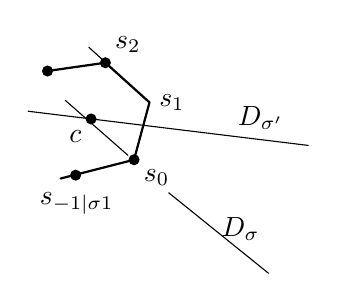
\begin{tikzpicture}[x=.7cm,y=.7cm,line cap=round,line join=round]
\draw[thick] (.35,3.55)--(1.40,3.7)--(2.2,2.98)--(1.92,1.94)--(.59,1.60);
\draw (.0,2.82)--(5.08,2.20) node[pos=.83,above] {$D_{\sigma'}$};
\draw (.67,3.02)--(1.81,2.02);
\draw (2.55,1.34)--(4.36,-.12) node[pos=.72,above] {$D_\sigma$};
\draw (1.10,3.98)--(1.52,3.60);
\foreach \x/\y in {.35/3.55,1.40/3.7,1.92/1.94,.86/1.66,1.14/2.68}{\fill (\x,\y) circle (2pt);}
\node[above right] at (1.40,3.7) {$s_2$};
\node[right] at (2.2,2.98) {$s_1$};
\node[below right] at (1.92,1.94) {$s_0$};
\node[below] at (.88,1.52) {$s_{\unsure{-1|\sigma1}}$};
\node[below left] at (1.14,2.65) {$c$};
\end{tikzpicture}}

[Nb \deleted{\unsure{à trouver}} $D_{\sigma'}$ est l'ens des pts fixes de $\sigma'$] -- On trouvera que les conditions à imposer à $\varphi$ pour qu'il y ait $s_0$ satisfaisant ttes les conditions impliquent que \deleted{\unsure{$D_{\sigma'}$}} $\sigma'$ est également une réflexion et $D_\sigma\ne D_{\sigma'}$ -- donc \deleted{\unsure{pour}} celà exclut \inserted{\text{a priori}} en plus un pt $c$ (le \uline{centre} du polygône \inserted{\text{qui est un pt fixe \unsure{sous|pour} $\varphi(D_n)$}}) parmi les pts éligibles pour $s_0$. On trouvera de plus que (pour $\varphi$ fixé, \deleted{les ens des pts $s$} \inserted{\text{\uline{admissible}}}) l'ens des $s_0\in\deleted{\unsure{tels}}D^{\sigma *}$ $=$ \deleted{distincts de} $D^\sigma-\{D\cap D^\sigma\}$ \deleted{\unsure{est un}} -- sur le quel le commutant \inserted{\text{$G$}} de $\varphi(\Gamma)$ dans $\mathrm{Aff}(E)$ opère de façon évidente) est un \uline{torseur} sous $G$.
% archive sheet number: 17

\scanpage{19}
% slanted
\margin{\uline{intercalaire}}
\uline{Proposition 3} (Sous réserve qu'on sache -- ou suppose -- que $\sigma'$ est une réflexion \deleted{d'\unsure{axe}} miroir $D_{\sigma'}\ne D_\sigma\unsure{\}}$ -- ce qui ne fait rien autre que la condition unimodulaire!) :

$1^\circ)$ Supposons $D_\sigma\cap D_{\sigma'}\ne\varnothing$, soit $c$ l'unique pt de $D_\sigma\cap D_{\sigma'}$, \deleted{\unsure{à $\varphi$|Alors}} Alors \deleted{\unsure{pour un anneau}} $c$ est l'unique pt fixe de $E$ sous $\Gamma$. Si on prend $c$ comme origine -- de sorte que $E$ devient un vectoriel, $\Gamma$ opérant linéairement --. Le groupe \inserted{\text{$G$}} des autom de $(E,\Gamma,\varphi)$ (i.e. le commutant de $\Gamma$ dans $\mathrm{Aff}(E)$ ou $\mathrm{Gl}(E)$) est égal au groupe des \deleted{\unsure{scalair}} homothéties non nulles, i.e.
\[
k^*\simeq G
\]
-- donc \deleted{$G$ opère \unsure{de façon simplement}} \inserted{\text{$D_\sigma^*$ est un $G$-torseur.}}

\deleted{\unsure{1}}\ $2^\circ)$ Supposons $D_\sigma\parallel D_{\sigma'}$. Soit $T\subset V={}$espace des translations le \deleted{\unsure{droite|droite ?}} \inserted{\text{1-vectoriel}} direction commune de $D_\sigma$ et $D_{\sigma'}$, et identifions $T$ \inserted{\text{$(\simeq k^{\unsure{*|+}})$}} \deleted{au} \inserted{\text{un}} sous-groupe de $\mathrm{Aff}(E)$ (ss-groupe du groupe des transl\unsure{tions|t\textsuperscript{ons}|ations}).
% archive sheet number: 18

\scanpage{20}
Alors $G=T$, donc ici encore \deleted{\unsure{$G$}} $D_\sigma^*=D_\sigma$ est un $G$-torseur

\uline{Dém} Il est évident dans l'un et l'autre cas que \inserted{\text{$G_0={}$}} $k^*$ resp $T$ $(\simeq k^{+})$ commute à $\sigma$ et $\sigma'$, donc à $\Gamma$ (engendré par $\sigma$ et $\sigma'$) donc
\[
\deleted{k^*}G_0\subset G\qquad\deleted{\text{resp } T\subset G}.
\]
Or $\deleted{k^*}G_0$ est transitif sur $D_\sigma^*$ \deleted{\unsure{g}} (dans l'un et l'autre cas) et comme $G$ \deleted{est} opère librement sur $D_\sigma^*$ \inserted{\text{grâce à \unsure{prop 1 ou 2}}}, il en résulte ``formellement'' que $G$ opère transitivement -- donc $D_\sigma^*$ est un $G$ torseur -- et que $G_0=G$, cqfd
% archive sheet number: 19

\scanpage{21}
[P. ex. dans le cas où $c$ existe \inserted{\text{-- qu'on prendra pour origine --}}, $G$ est l'ens des homothéties de centre $c$ (isomorphe à $k^*$) qui est évidemment simplement transitif sur l'ens des pts de la droite \unsure{homogène} \uline{épointée}.]
% slanted
\margin{c'est le cas \deleted{\unsure{ssi}} $n\ne\operatorname{car} k$ \deleted{\unsure{$n\ne p$}} et $n\ne4$ si $p=2$ (ou $6$)}
\inserted{\text{En fait il est clair \inserted{\text{a priori}} que $G$ opère librement, à cause \deleted{du} cor \unsure{?} \deleted{\unsure{(prop)}} de la prop. 1. Donc \deleted{\unsure{le montrer plus court}} la question est celle de la transitivité\ldots}}
% slanted
\margin{on trouve déjà que $k^*=G$ dans le cas où $c$ ``existe'' (i.e. centre pas à l'infini!) Dans le cas $D_\sigma\parallel D_{\sigma'}$, on \deleted{\unsure{trouvait}} translations de direction $D_\sigma$ commutent à $\deleted{\unsure{D}}\sigma,\sigma'$ d'où la conclusion}

\uline{Cor 1}) Deux $n$-polygônes réguliers \deleted{\unsure{g}} \unsure{épinglé|épinglés}, tels que les représentations correspondantes de $D_n$ soient isomorphes, sont isomorphes. (la réciproque étant triviale). Donc la classific\unsure{ion|ation} mod isomorphismes des représentations affines \inserted{\text{admissibles}} de dim $2$ de $D_n$ (sur $k$ corps fixé) équivaut à celle des $n$-polygônes réguliers.

\uline{Cor} $2)$ Soit
\[
\begin{aligned}
\varphi &:D_n\mathbin{\unsure{-|\to}}\mathrm{Aff}(E)\\
\varphi' &:D_n\mathbin{-}\mathrm{Aff}(E')
\end{aligned}
\]
deux repr. admissibles, et soit $P$ un polygone \unsure{$n$-régulier|$n$régulier} subordonné à $\varphi$ (dont la donnée équivaut à celle d'un $s_0\in D_\sigma^*\ldots$). Alors si à tt isom $\Theta:(E,\varphi)\to(E',\varphi')$ (isom. affine \deleted{\unsure{deux}} tel que $\Theta\varphi(g)\Theta^{-1}=\varphi'(g)$ $\forall g\in D_n$) on associe le polygône régulier \deleted{\unsure{sub}} $P'=\Theta(P)$, subordonné à $P'$, on
% archive sheet number: 20

\scanpage{22}
trouve une \uline{bijection} \inserted{\text{($1^\circ)$ disait que c'était une surjection)}} entre l'ens \deleted{des} \deleted{\unsure{is.|isom.}} $\mathrm{Isom}((E,\varphi)(E',\varphi'))$ et l'ens des $n$-pol rég. \inserted{\text{ép.}} subordonnés à $\varphi'$.

De façon suggestive, on peut dire que la donnée d'un polygône $n$-régulier subordonné à une repr. $\varphi$ admissible -- ou ce qui revient au $=$, le choix d'un pt $s\in D_\sigma^*$) revient à la donnée d'un \uline{épinglage} de $\varphi$ (ayant comme effet d'éliminer les autom -- car $G$ opère librement sur $D_\sigma^{\unsure{*|\wedge}}$ -- sans introduire de nouvelles classes d'isom. -- car $G$ opère transitivement --).
% archive sheet number: 21

\scanpage{23}
\textcircled{\small IV} Où on laisse tomber la condition de fidélité.

Considérons des données (11) satisfaisant (13) mais pas néc. (12) ; donc à part l'unimodularité, on laisse tomber la condition $\varphi$ fidèle. Que se passe-t-il ?

\uline{Proposition 4} \inserted{\text{Sous les conditions précédentes}} \deleted{Pour que $\varphi$ soit fidèle, il faut et}

(a) Si $v\in D_n^0$ i.e. $v=u^i$, alors $v_E=\mathrm{id}\iff v(s_0)=s_0$.

(b) Pour que $\varphi$ soit fidèle, il f et s. que $\varphi\mid D_n^0$ soit fidèle, \deleted{i.e. que} \inserted{\text{ou encore}} (par a)) que $u^i s_0=s_0\Longrightarrow i\equiv0\ (n)$ (i.e. $u^i=1$), ou encore que $\forall d\in{\mathbb N}^*$, $d\mid n$, on ait $u^d(s_0)\ne s_0$ \unsure{$N$|$\mathcal N$}

(c) \deleted{Soit} Le noyau de $\varphi$ \deleted{\unsure{$G$}} est \deleted{un sous-groupe de} engendré par un (unique) élément $u^{\deleted{\unsure{i}}d}$, où \deleted{$i$ est} $d$ est un diviseur de $n$ tel que \deleted{$d\geq3$. \unsure{--} de sorte que $\varphi$ \unsure{est induit une repr. fi}} \inserted{\text{$n'=n/d\geq3$}}

\uline{Dém} (a) $v_E=\mathrm{id}\iff v(s_{\nu})=s_\nu\ \forall\nu$ (car les $s_\nu$ engend\textsuperscript{t} aff\textsuperscript{t} $E$) or $s_\nu=u^\nu s_0$ donc $v(s_\nu)=vu^\nu s_0=u^\nu v s_0$, donc il suffit $v(s_0)=s_0$.
% archive sheet number: 22

\scanpage{24}
(\unsure{c|b}) \deleted{\unsure{Soit}} Le noyau de $\varphi\mid D_n^0$ est un sous gpe de $D_n^0=Z/n\mathbb Z$, donc \deleted{de la} c'est le ss-groupe engendré par un $u^i$ où $i$ est un diviseur \unsure{unqt|un\textsuperscript{t}|$>0$} déterminé de $n$ -- \deleted{\unsure{c|et}} qui a priori pourrait être $1$ ou $2$. Mais si \deleted{\unsure{$n=$|$i$}} $n'$ est tel que
\[
n=n'd
\]
\deleted{$\varphi$ se factorise en}
\[
\deleted{\varphi':D_{n'}\mathbin{\unsure{-|\to}}\mathrm{Aff}(E)}
\]
on voit que \deleted{$S$ a un} $\operatorname{card}S=n'$, \deleted{donc} et comme $S$ engendre aff\textsuperscript{t} $E$, on aura $n'\geq3$. Enfin, comme $\varphi$ se factorise par
\[
\varphi':D_{n'}\mathbin{\unsure{-|\to}}\mathrm{Aff}(E)
\]
avec $\varphi'\mid D_n^0$ \unsure{$^{\bullet}$} fidèle -- et que les conditions (\unsure{1|11}) sont évidemment satisfaites aussi pour $\unsure{\rho'|\varphi'}$ -- (b) implique que $\varphi'$ est fidèle, donc $\operatorname{Ker}\varphi^{\unsure{\prime\prime|\circ}}$ est ident à $\operatorname{Ker}(\varphi\mid D_n^0)$.

\margin{se montre avant (c)}
(b) \deleted{\unsure{Résulte du|Résulte de}} \deleted{Supposons $\varphi\mid D_n^0$ fidèle.} Équivaut au
% archive sheet number: 23

\scanpage{25}
\uline{Corollaire} 1 Si $v\in D_n^{\deleted{\unsure{*}}}\smallsetminus D_n^0$, alors $\varphi(v)\ne\mathrm{id}_E$

En effet, \deleted{\unsure{$\varphi(v)$}} il est clair que $\varphi(v)$ échange les deux ordres circulaires \inserted{\text{$\{v_E\mid v\in\unsure{w|\omega|u}\}$}} sur $S$, \deleted{distincts des \unsure{propriétés postulées}} \deleted{\unsure{et|donc} $v_E$} donc ne peut être l'identité sur $S$, donc pas non plus sur $E$.

\uline{Corollaire 2} Considérons \deleted{\unsure{le|la}} l'entier $n'$ comme \inserted{\text{dans (b)}} dessus. Alors \deleted{$\varphi':D_{n'}$}
\[
\left\{\begin{aligned}
\varphi' &:D_{n'}\longrightarrow\mathrm{Aff}(E)\\
s_0&\in E
\end{aligned}\right.
\]
définissent dans $E$ un polygône épinglé à $n'$ côtés.

\uline{Scholie} On peut considérer que la donnée $\{\varphi,s_0\}$ correspond à une réalisation géom du polygone comb. type $\Pi_0(n)$, qui est un \uline{revêtement à $d$ feuillets} de la réalisation géom \inserted{\text{$(\varphi',s_0)$}} du polyg. comb. type $\Pi_0(n')$. Quand on fera des calculs avec un
% archive sheet number: 24

\scanpage{26}
$n$ fixé, on trouvera \inserted{\text{d'abord}} des \deleted{\unsure{cas}} repr. $\varphi:D_n\to\mathrm{Aff}(E)$, sans savoir d'avance quand elles sont fidèles -- ce \unsure{sera|serait} là une question d'un \inserted{\text{tout}} autre type que les précédentes \deleted{\unsure{à}} \inserted{\text{(satisfaire $12\ 2^\circ$,}} trouver $s_0$ satisfaisant les conditions (13)), demandant une analyse plus \deleted{détaillée} délicate de la situation. Surtout quand on regardera des réalisations géom. d'un $\Pi_0(n)$ sur un anneau plus général qu'un corps (tel que $\mathbb Z$ -- ou \deleted{plus} mieux, les anneaux \inserted{\text{tels que $\mathbb Z[T]/(T^n-1)$ ou les anneaux}} cyclotomiques -- on trouvera \unsure{souvent} \deleted{que} \inserted{\text{pour les fibres en}} ttes les car. sauf un nb fini (y compris en car zéro) une repr. fidèle, tandis qu'en certaines caractéristiques \unsure{elles|elle} devient non fidèle (infidèle ?)) -- elles n'en cessent pas
% archive sheet number: 25

\scanpage{27}
pour autant d'exister, et de définir des polygônes réguliers en ces car. exceptionelles, mais à un nb plus petit de cotés (divisant $n$). Ce serait \unsure{empoisonnant|emprisonnant} -- et \inserted{\text{finalement tout à fait}} artificiel -- de traîner tout au long du chemin la condition de fidélité, au lieu de se borner à l'examiner seulement aux moments \deleted{voulus} où cette considération est utile.

\textcircled{V} \deleted{\unsure{Abandon de $n$}} \uline{Cas des $\infty$-polygônes}

On peut aller encore plus loin, en notant que la donnée de (11) (a) revient à la donnée de
\[
\deleted{\unsure{a}}\quad
\left\{\begin{aligned}
&\sigma_E,\sigma'_E\in\mathrm{Aff}(E)\qquad\text{satisfaisant}\\
&\sigma_E^2={\sigma'_E}^2=\mathrm{id}_E,\quad
(\underbrace{\sigma'_E\sigma_E}_{u_E})^n=\mathrm{id}_E
\end{aligned}\right.\tag*{(14)}
\]
\deleted{satisfaisant} \deleted{(15) $s_0$} \deleted{Et la fidélité signifie que (étant don-} \deleted{\unsure{$s_0$}} \unsure{Etant|Étant} donné $s_0$, \deleted{la fidé} satisfaisant

\[
\deleted{(15)}\quad
\left\{\begin{aligned}
&\sigma_E s_0=s_0\\
&s_0,\ \deleted{\unsure{\sigma'_E\sigma_E s_0=u}}\,s_1=u_E s_0\text{ et }\inserted{s_2={}}u_E^2s_0\\
&\hspace{43mm}\text{sont non alignés}
\end{aligned}\right.\tag*{(13)}
\]
% archive sheet number: 26

\scanpage{28}
la condition de fidélité s'écrit
\[
\forall\ \text{diviseur }d\mid n,\quad\text{on a }\inserted{u_E^d\ne\mathrm{id}\ \text{i.e.}}\quad u_E^d(\deleted{\unsure{=}}s_0)\ne s_0
\tag*{(15)}
\]
(cf prop 4 (b)) -- et il suffit \inserted{\text{$=$}} de l'exiger pour $3\leq d\leq\left[\frac n3\right]$ (donc si $3\leq n\leq8$, cette condition est automatiquement satisfaite, le premier entier où elle ne l'est pas est $n=9$, où il suffit de \inserted{\text{\unsure{le}}} tester pour $n=9$ -- le $9$-gone régulier peut \deleted{\unsure{consis}} dégénérer pour consister trois fois un $3$-gône régulier --) -- Mais de $=$ qu'on peut laisser tomber cette condition de fidélité, on peut laisser tomber la \inserted{\text{dernière}} condition (14)
\[
(\sigma'_E\sigma_E)^{n}=\mathrm{id}_E
\]
ce qui signifie qu'on regarde en fait une représentation
\[
\varphi:D_\infty\mathbin{\unsure{-|\to}}\mathrm{Aff}(E)\tag*{(16)}
\]
du groupe diédral infini, sans se préoccuper si elle se factorise par $D_n$ ou non -- étant entendu que l'
% archive sheet number: 27

\scanpage{29}
on s'intéressera plus particulièrement, pour des entiers $n$ convenables, aux repr. de $D_\infty$ qui veulent bien se factoriser par $D_n$. C'est dire que, \deleted{\unsure{le}} de ce point de vue, la question de fidélité ne se pose plus -- les représentations les plus intéressantes \inserted{\text{pour nous}} de $D_\infty$ \deleted{étant} -- celles qui donnent naissance aux \deleted{\unsure{correspondent}} polygônes réguliers finis -- étant précisément non fidèles!

% slanted
\margin{\uline{Pt de vue} $\Pi$-\uline{épinglé} $\Pi$ polygone comb. quelconque (fini ou infini)}
Arrivé à ce point, il y a lieu de considérer -- de $=$ que des polygônes \uline{combinatoires} infinis \inserted{\text{$\Pi=(S,\omega)$ --}} (tout comme les poly comb. finis) des réalisations \inserted{\text{ou \uline{repr.}}} géom de ceux-ci (pas néc. fidèles), et de $=$ des repr. géométriques \uline{régulières}, \deleted{en exigeant pour ces dernières} \deleted{\unsure{Une réalisation}} \deleted{en exigeant \unsure{pour} ces dernières} \deleted{que} % slanted
\margin{\uline{Déf}} On entendra par là une
% archive sheet number: 28

\scanpage{30}
réalisation géom satisfaisant \unsure{la condition|les conditions} :
\[
\begin{aligned}
&\deleted{\unsure{\exists}}\ \forall v\in\mathrm{Aut}(\Pi),\quad\exists\unsure{1|!}v_E\in\mathrm{Aut}(E)\\
&\text{telle que }\quad v_E(\varphi(s))=\varphi(v(s))
\end{aligned}\tag*{(17)}
\]
\diagram{\begin{tikzcd}[ampersand replacement=\&]
S\arrow[r,"\varphi"]\arrow[d,"v"'] \& E\arrow[d,"v_E"']\\
S\arrow[r,"\varphi"] \& E
\end{tikzcd}}

\deleted{Ce qui} La donnée d'une telle réalisation revient à la donnée
\[
\left\{\begin{aligned}
a)\ &\varphi_\Gamma:\Gamma=\mathrm{Aut}(\Pi)\longrightarrow\mathrm{Aff}(E)\\
&v\longmapsto v_E\qquad\text{hom de groupes}\\
b)\ &S_{\deleted{\unsure{E}}}\xrightarrow{\varphi_S}\deleted{\unsure{S_E\subset}}E\quad
\text{\deleted{(\unsure{entre|entre les}}application compatible \deleted{\unsure{sur}} avec \deleted{\unsure{ce}} les\deleted{)}}\\
&\hspace{48mm}\text{op. de }\Gamma
\end{aligned}\right.\tag*{(18)}
\]
satisfaisant les \inserted{\text{seules}} conditions supplémentaires
\[
\deleted{\unsure{(1^\circ)|(19)}}\quad S_E\text{ n'est pas contenu dans une droite}\tag*{(19)}
\]
\deleted{$\unsure{b)}\ \unsure{(2^\circ)|(20)}$}

Si on se \deleted{fixe} donne $i_0\in S$, et si $\sigma_{0\deleted{\unsure{s_0}}}$ désigne l'unique \deleted{\unsure{aut}} él. de $\Gamma$ $\ne1$ tel que \deleted{$\sigma_0s_0=s_0$,}
\[
\sigma_0\ne1_\Gamma,\quad\sigma_0 i_0=i_0\tag*{(20)}
\]
la donnée de $\varphi_S$ équivaut \inserted{\text{(pour $\varphi_\Gamma$ donné)}} à la donnée de
\[
\left\{\begin{aligned}
&s_0\in E\qquad[\,s_0=\varphi_S(i_0)\,]\\
&\text{satisfaisant}\quad \sigma_0s_0=s_0
\end{aligned}\right.\tag*{(21)}
\]
et la condition (19) équivaut alors, \deleted{\unsure{si}} \inserted{\text{si on choisit $u\in\omega$}}
\[
\deleted{s_0\ne s_1,\ s_2={}}\ s_0,s_1=u_Es_0,s_2=u_E^2s_0\quad\text{non alignés}.\tag*{(22)}
\]
% archive sheet number: 29

\scanpage{31}
Mais la donnée de $(s_0,u)$ équivaut à celle d'un \uline{répère} de $\Pi$, i.e. d'un isom \deleted{entre $\Pi$ et}
\[
\Pi\simeq\Pi_0(n)
\]
(où $n$ \deleted{\unsure{$\in\mathbb N^*$}} est un entier $\geq3$ \uuline{ou $+\infty$}), et la donnée de a) \deleted{\unsure{b)|a)}} équivaut donc à la donnée de (14) (sauf la dernière \deleted{\unsure{relation|condition}} \inserted{\text{condition de (14) si $n=+\infty$}}), \deleted{et} celle de (b) équivaut à la donnée de $s_0\in E$ satisfaisant la \deleted{première} relation $\sigma_{\deleted{\unsure{0}}E}s_0=s_0$, et la condition (19) se traduit par (22). En résumé

\uline{Prop} 5 Les \deleted{repr.} réalisations géom \inserted{\text{\uline{régulières}}} de $\Pi_0(\infty)$ \inserted{\text{dans $E$}} correspondent aux \deleted{couples} triples $(\sigma_E,\sigma'_{E\deleted{\unsure{*}}},s_0)$ de deux autom affines \deleted{et} \inserted{\text{de $E$}}
\[
\deleted{\unsure{\sigma}}\qquad\sigma_E,\sigma'_E\in\mathrm{Aff}(E)
\]
et d'un \deleted{$s_0\in E$, satisfaisant les}
\[
s_0\in E
\]
satisfaisant les conditions
\[
\begin{aligned}
(1^\circ)\quad &\sigma_E^2={\sigma'_E}^2=\mathrm{id}\\
(2^\circ)\quad &\sigma_Es_0=s_0\\
(3^\circ)\quad &\deleted{\unsure{(1,2,3)}}\ \deleted{\unsure{(u_E=\sigma'_E\sigma_E}}\ 
s_0,s_1=u_Es_0,s^{\deleted{\unsure{2}}}_2=u_E^2s_0\quad\text{non alignés}
\end{aligned}
\]
(\deleted{où} \inserted{\text{où on a}} \deleted{\unsure{$u$}}\inserted{\text{posé}}
\[
u_E=\sigma'_E\sigma_E
\]
% archive sheet number: 30
